%% ---------------------------------------------- Exploring Some OSNs
\section{Exploring Specific Online Social Networks}

In this section we are going to explore in greater detail some of the \glspl{osn} presented
in Table \ref{table:osns}. The selection of the social networks was not aleatory, we are going
to study deeply the \glspl{osn} that gather some important characteristics, that will be of use in
the future when we design the system for analyzing and visualizing social networks. First, the
\gls{osn} must be accessible, this said, one must be capable of extracting information from the platform
in order to analyze it. Second, the \glspl{osn} must be the most diversified as possible, so that we
can draw different types of conclusions derived from different kind of analysis, for then give proof
of the adaptability of the system to different \glspl{osn}. Considering the previous
comments, these are the following \glspl{osn} that will study with more detail:
\begin{itemize}
  \item Facebook
  \item Instagram
  \item LinkedIn
  \item ResearchGate
  \item Pinterest
\end{itemize}

%% ---------------------------------------------- Exploring Some OSNs
%% -------------------------------------------------- Facebook
\subsection{Facebook}

Facebook is an \gls{osn}, created by Mark Zuckerberg in 2004, which started out by being an exclusive social network for Harvard students, but came later to spread across
the country and the globe, having today more than one billion users.\\
\indent Before diving into details of Facebook's domain, one must first point out some of its general aspects. Facebook basically allows anyone with a valid email address to create a public and personalized profile,
we say personalized in terms of displayed content or information such as profile photo, name, work, homeland, education etc. .
The next fundamental step is connect with other users, by sending friendship requests to other Facebook users (this are bidirectional relations).
The base entity of the network is the user, but entities such as brands, companies can also be part of the platform, appearing normally
in the form of page, being a page a public place inside the network with marketing or business related purposes (celebrities, public institutions also use pages as form of appearing in Facebook).\\
\indent The next parts of this section will clarify the roles of this entities and their way of interact with each other, also other important concepts will be presented.

\subsubsection*{Domain Model}

\begin{figure}[h!]
  \hspace*{-1in}
  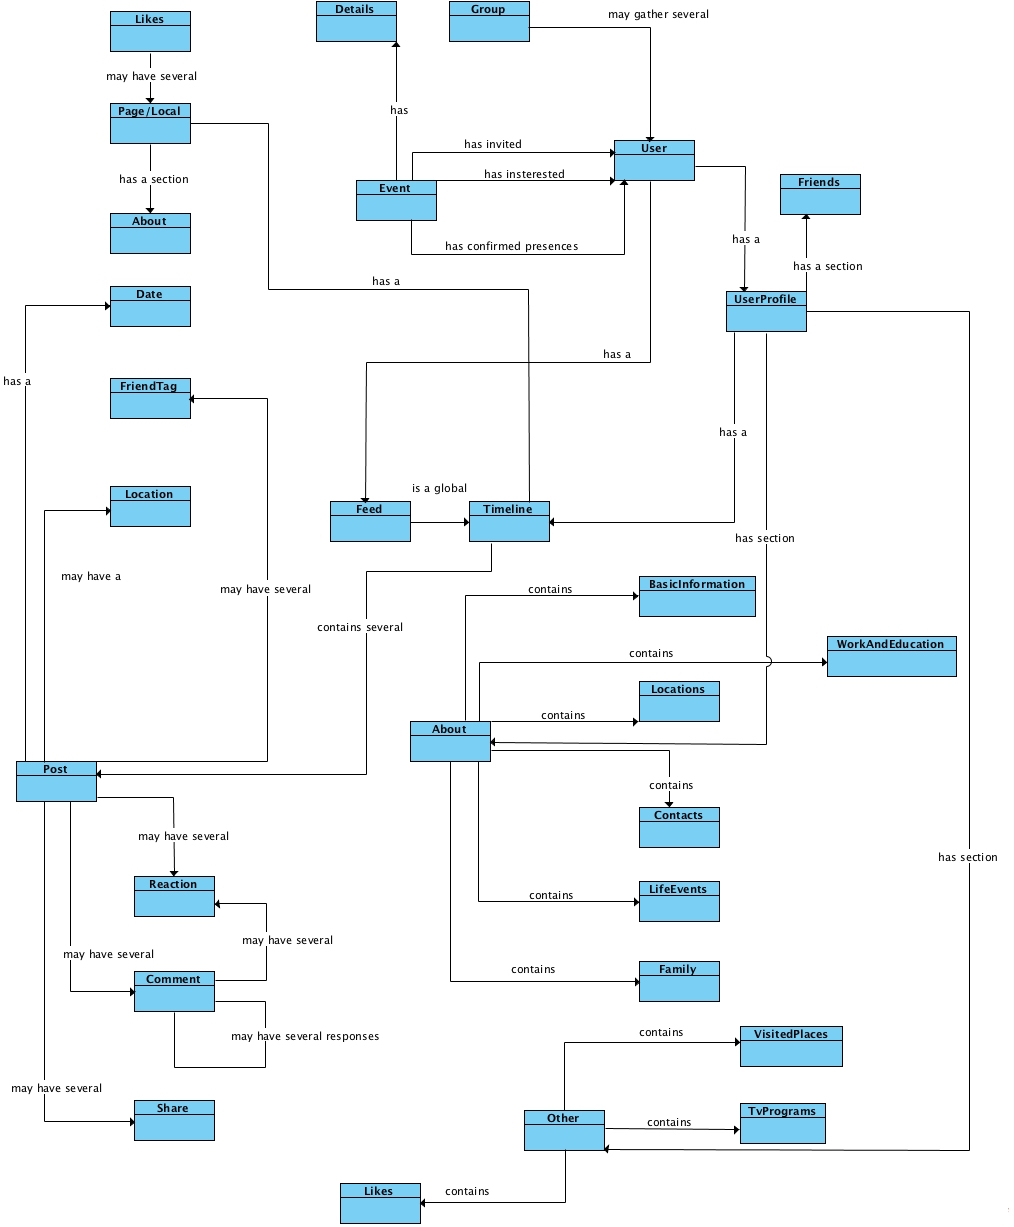
\includegraphics[width=1.28\textwidth]{img/facebook-domain-model.jpg}
\caption{\label{img:fbdomain} Facebook domain model schema.}
\end{figure}

\indent In this section we explore the domain of Facebook represented in Figure \ref{img:fbdomain} in detail, what are the pieces that conceptually build
this platform, and how they relate. The schema in Figure \ref{img:fbdomain} represents a macroscopic perspective among Facebook components and their organization.\\
\indent There are two entities with bold labels in the schema, this are, \textbf{User} and \textbf{Post}, being
\textit{User} the base entity in the network (the node in the network graph basically), and \textit{Post} the most basic unit of content sharing in Facebook.\\
\indent Facebook is interesting in terms of data gathering, because despite offering users' basic information
and to whom that users are related (\textit{Friends} box), it has a collection of other interesting data
such as the family relationships (\textit{Family} box), geographical locations where the user lives, or
visited locations (\textit{Locations} and \textit{VisitedPlaces} boxes respectively), and among other things, user information
may contain the personal interests that were explicitly inputed by the user (\textit{Likes} box).\\
\indent In what concerns to user activity in the platform, the \textit{Timeline}, provides all the user
Posts chronologically ordered, this is where Facebook dynamism takes place, users are constantly
adding content to their timeline, it may be life related events or simply sharing other users posts linking content. The user feed (\textit{Feed} box) represents
a global timeline where the user can consult all the posts on his network (this is by default the user's landing page on the platform).\\
\indent Facebook has, with time, become more then a user profile centralized network, it has invested in expand its horizons, becoming
the place where pages of brands, companies, organizations (media, political, non-profitable etc.), or places (cities, monuments, bars etc.) live (\textit{Page/Local} box).
This entities that are now cohabiting with users in the Facebook ecosystem, take advantage of the platform and its range to get their updates to most people as possible. The profile
for these pages are in many ways different form the user's profile, it also has a timeline, but the about information and other details represent a smaller part of page's profiles,
the most important metric for pages is its number of \textit{likes} (\textit{Likes} box), it represents the number of users in the network that follow the page, it might be users
that simply have a certain relation with the entity or simply want to keep in touch by regularly receiving these entities updates in their Facebook walls
\footnote{Facebook wall an area where users can see the posts of their friends and/or liked pages, in a chronological order}.\\
\indent Other Facebook entities not yet mentioned, are events (\textit{Event} box). These are events inputed in the platform that allow
users to keep updated about relevant events happening mainly in their area. Users can tag the event as \textit{interested in}, showing their friends
the will of participating in some event, or they can simply reject the event. Users also can confirm participation on events
showing their network that they will be present. Events keep three separated counters for users, they count the number of invited users, number of
interested users and number of confirmed users (these relations are expressed as links between the \textit{Event} box and the \textit{User} box).\\
\indent In Facebook is also possible to join groups of users, this groups may be public or private, and they generally are focused on a specific matter,
or gather users from one same institution or organization (e.g. Facebook group of students of the University of Minho).
Having this feature of groups, clustering users by they interests one may say that groups, some way, transform Facebook in a "multi interest-based \gls{osn}".

\subsubsection*{Facebook Graph API}
Facebook has today several software \textit{kits} for developers to interact with the platform in the most diversified and imaginable ways. Facebook developers
offers a range of variated software products that vary from monetization programs, that focus on how to make users profit from Facebook, Analytics to developers who
have their apps embedded in the Facebook platform understand their audience and the performance of their apps, etc. (\cite{fbproducts}).\\
\indent In this master's thesis context, the relevant software that Facebook has available is the Facebook Graph API. This API basically allows developers to collect information
from Facebook such as posts, photos, videos, pages etc. According to \cite{fbgapi}, the common scenarios for using the Graph API
are the following: determine whether two people are friends on Facebook; publishing new status and updates, uploading content (photos, video etc.); sharing links. But in this project what we seek is
build the most biggest and detailed network as possible, with analysis and visualization purposes in mind.\\
\indent For building the network fetching users friends information is crucial, this was possible until Facebook Graph API v2.0 (trough the router \textit{/me/friends}), one could actually retrieve
friends information and build a network from there. From v2.0 on, to achieve what was explained before, one must request a special permission called \textbf{user\_friends}
from each user. The permission \textbf{user\_friends} is no longer included by default in every login. This change breaks down the possibility of gather Facebook information via its Graph API,
this said, we need in the future to look up alternative paths to extract data from Facebook.


%% ---------------------------------------------- Exploring Some OSNs
%% -------------------------------------------------- Instagram
\subsection{Instagram}

\begin{quote}
\textit{"Since the beginning, Kevin has focused on simplicity and inspiring creativity through solving problems with thoughtful
product design. As a result, Instagram has become the home for visual storytelling for everyone from celebrities, newsrooms and
brands, to teens, musicians and anyone with a creative passion."} \cite{instabout}
\end{quote}

Similarly to Facebook we are going to explore Instagram in the same way. Instagram was originally developed by Kevin Systrom and Mike Krieger, and launched in 2010, only
for iPhone devices. Within a year Instagram was able to gather around 10 million of users. Later, in 2012 Facebook acquire Instagram for approximately 1 billion dollars.\\
\indent As already mentioned in Table \ref{table:osns}, does not belong to the group of general purpose \glspl{osn}, instead, Instagram specially focused on photo
and video sharing, building a global community that shares more than 95 million photos every day.\\
\indent According to \cite{instabout}, since
the very beginning Instagram was a very simplistic platform, being this characteristic reflected on its domain model.

\subsubsection*{Domain Model}

\begin{figure}[h!]
  \hspace*{-1in}
  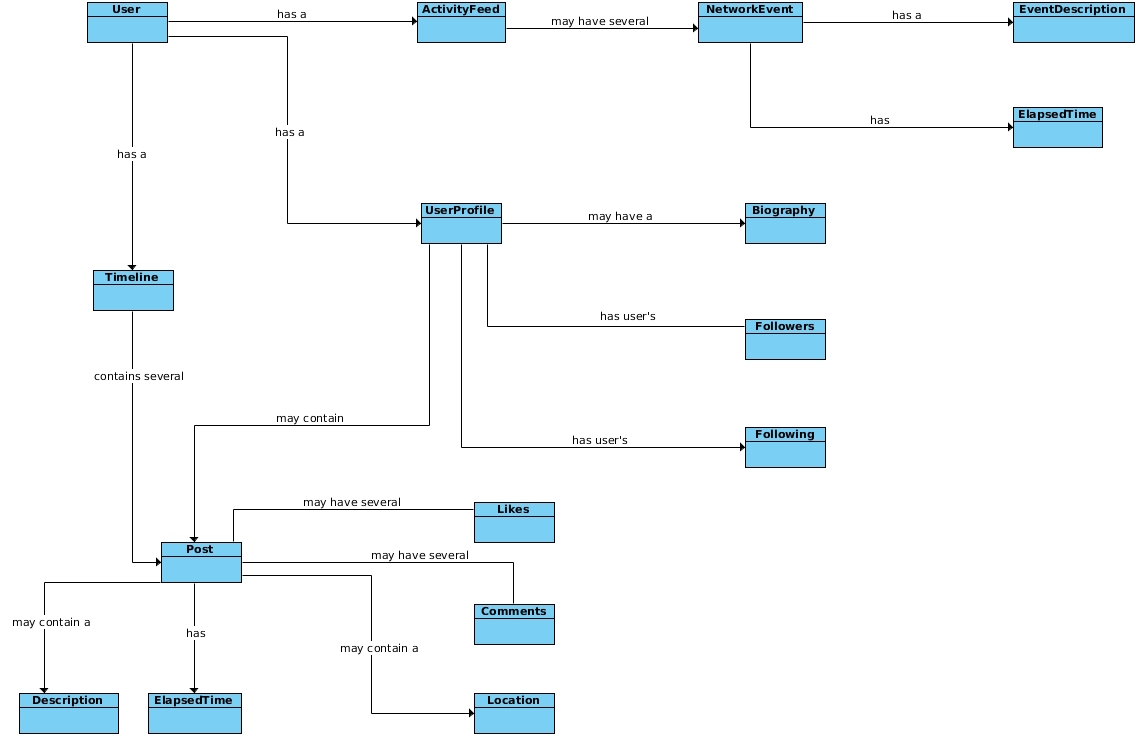
\includegraphics[width=1.28\textwidth]{img/instagram-domain-model.jpg}
\caption{\label{img:instadomain} Instagram domain model schema.}
\end{figure}

Figure \ref{img:instadomain} represents the domain model of Instagram, and as we can observe, simplicity its the essence of this platform, since this diagram is far
more a realistic representation of Instagram than Figure \ref{img:fbdomain} is a representation of Facebook, and this may be why Instagram is so massively adopted by users
on the Internet, because it goes directly to the point, focusing mainly on sharing activity, offering a real easy and simple user experience.\\
\indent Now concerning to the domain model, we can see that a user and its profile (\textit{User} and \textit{UserProfile} boxes) are very simple entities, because
a user's profile is only its biography (\textit{Biography} box), relationships (\textit{Followers} and \textit{Following} boxes) and the user's posts, that despite
being chronologically ordered, do not intend to form any kind of timeline such as Facebook, instead it represents more the concept of a wall with frames hanged on it.\\
\indent In Instagram the landing page, represents a timeline (\textit{Timeline} box) with posts from users we follow. Regarding to posts (\textit{Post} box), one can
comment posts (\textit{Comment} box), but one cannot react or respond to comments (this preserves simplicity even more, for nested comments represent
 a complex part of \gls{osn} such as Facebook), and react to them by the \textit{like} reaction (\textit{Like} box).

\subsection*{Instagram API Platform}
In consequence of a simple domain, Instagram API Platform, provides simple and useful
end points for programmatic publishing, and for network discovering, as far as concerning to this project, the late utility
is more of interest. Instagram allows to get users, their relationships and also the media shared content (posts).\\
\indent Similarly when exploring Facebook Graph API, we now found also very intimidating restrictions for the purpose of this project,
this restrictions include limited rate of 500 API requests per hour, and end point specific limitations that allow only to
perform 30 requests per hour to getting users' relationships data. (\cite{instadev})

%% ---------------------------------------------- Exploring Some OSNs
%% -------------------------------------------------- LinkedIn
\subsection{LinkedIn}

Moving on to the next \gls{osn} we now have LinkedIn. According to \cite{linkabout}, LinkedIn was launched officially on May 5 of 2003, and by the end of
that month, the network had already more than 4500 members. In 13 June of 2016 LinkedIn was acquired by Microsoft in an all-cash transaction valued at \$26.2
billion (\cite{microlink}).\\
\indent LinkedIn is an \gls{osn} that has a very narrow purpose, which is
connecting professionals around the globe to make them more productive and successful.

\subsubsection*{Domain Model}

\begin{figure}[h!]
  \hspace*{-1in}
  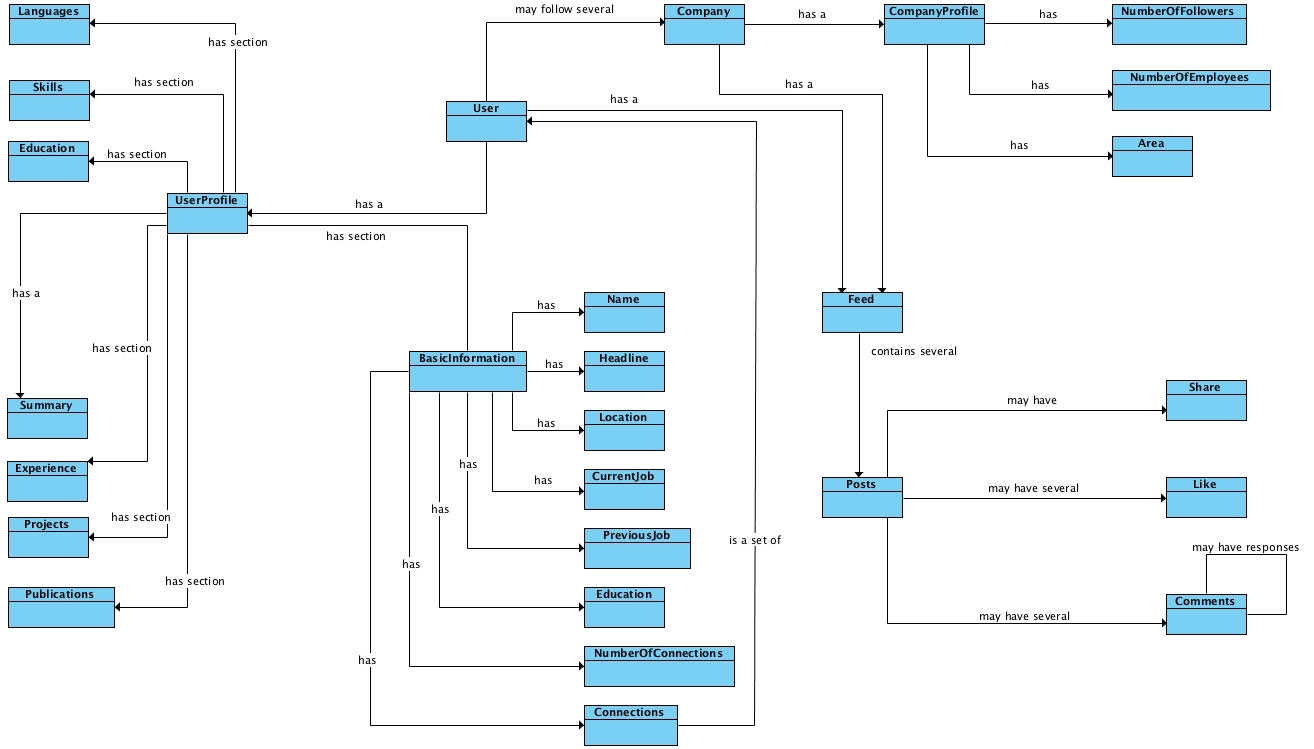
\includegraphics[width=1.20\textwidth]{img/linkedin-domain-model.jpg}
\caption{\label{img:linkdomain} LinkedIn domain model schema.}
\end{figure}

\indent Being a more purpose oriented \gls{osn} and focused on the professional
world, makes LinkedIn platform more complex, even with a simplified representation of the domain model, as we can observe in Figure \ref{img:linkdomain} it is schema
\footnote{\indent In the schema presented on Figure \ref{img:linkdomain}, much of the platform complexity was simplified in order to produce a simple domain, and to narrow
down this analysis to the core components and concepts of LinkedIn.}
far more complex that Instagram, having more or a similar complexity comparing to Facebook.\\
\indent In LinkedIn the user profile (\textit{UserProfile} box) is very rich in terms of what is important for building an individual professional image (profile),
starting by one individual's basic information (\textit{BasicInformation} box) that has information like name, location and current and/or previous jobs. Then
the user profile has several sections with very specific purposes such as professional experience (\textit{Experience} box), languages (\textit{Languages} box) or
education (\textit{Education} box), all this summed up give a very precise perspective of an individual's "professional appearence". At the bottom of the profile
we have along with the professional recommendations and connections, the skills or expertise section (\textit{Skills} box), this is one of the most attractive features
in the LinkedIn platform. Skills in LinkedIn are a tagging system that allow user's to expose their expertise trough their public profile and then receive feedback
on them according to their ability on that specific skill, this is a very important and promising feature for matching user's profiles with
job positions requirements.\\
\indent LinkedIn's main entities are not only users, the industry is massively represented in this network too. Companies may have a company profile
(\textit{Company} and \textit{CompanyProfile} boxes) where they present the company, containing basic information such as number of people following the company
number of employees (giving the idea of the company dimension) and the area where the company fits (pharmaceuticals, technology etc.) (\textit{NumberOfFollowers},
\textit{NumberOfEmployees} and \textit{Area} boxes respectively).\\
\indent Other important concept of LinkedIn is the user feed where the user can chronologically consult a series of posts produced by their connections
or by companies that their follow.

\subsection*{LinkedIn API}
LinkedIn provides a REST API (\cite{linkapi}), but still similarly to the \glspl{osn} we been studying its very limited. In what concerns to data retrieval LinkedIn only allows
the consult of basic profile data, this is the data retried from the LinkedIn interactive REST console:\\

\begin{verbatim}
  {
  "firstName": "Daniel",
  "headline": "Graduate Front-end Developer at Blip.pt",
  "id": "k_yk8W37WH",
  "lastName": "Caldas",
  "siteStandardProfileRequest":  {
    "url": "https://www.linkedin.com/profile/..."
  }
\end{verbatim}

\indent As we can see from the above data sample, we only could fetch some data properties, that would not bring value in terms of network analysis.

%% ---------------------------------------------- Exploring Some OSNs
%% -------------------------------------------------- ResearchGate
\subsection{ResearchGate}

\begin{quote}
\textit{"Founded in 2008 by physicians Dr. Ijad Madisch and Dr. Sören Hofmayer, and computer scientist
Horst Fickenscher, ResearchGate today has more than 11+ million members. We strive to help them make progress happen faster."} \cite{rgate}
\end{quote}

ResearchGate is an \gls{osn} built specifically for scientists, with the goal of easing the task of collaborative research around the globe. ResearchGate
strikes to connect the world of science and make research open to all.
\clearpage

\subsubsection*{Domain Model}

\begin{figure}[h!]
  \hspace*{-1in}
  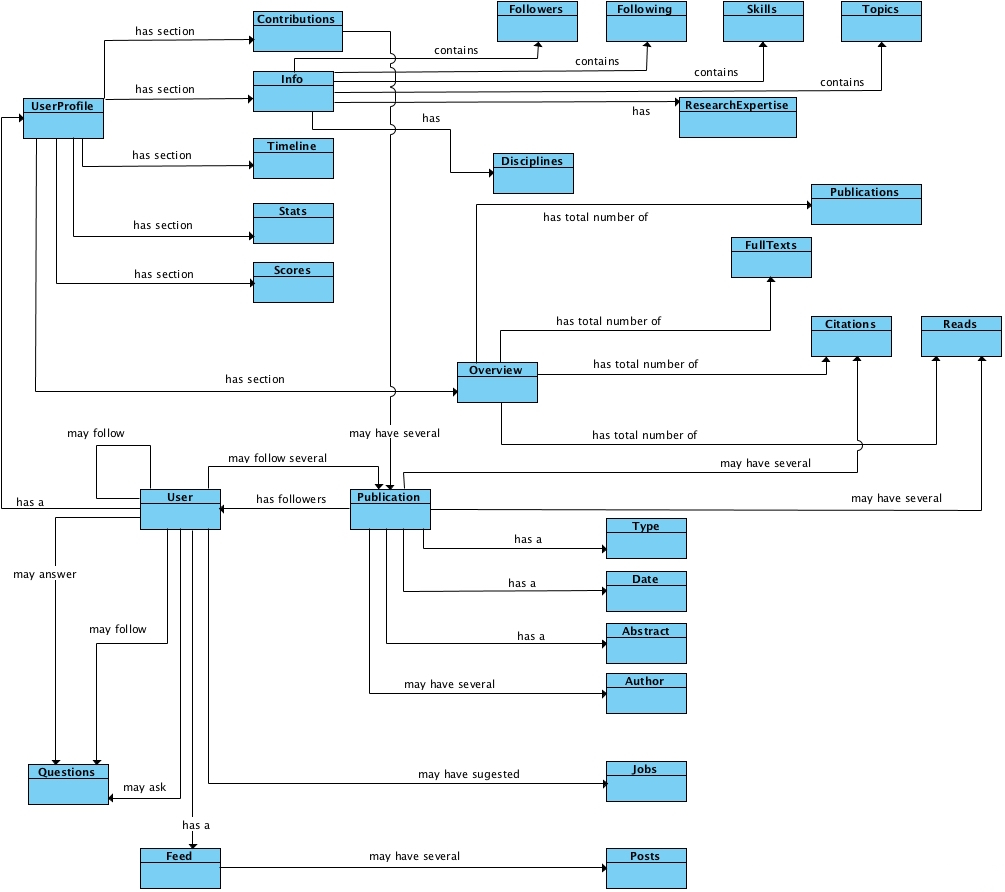
\includegraphics[width=1.20\textwidth]{img/researchgate-domain-model.jpg}
\caption{\label{img:rgatedomain} ResearchGate domain model schema.}
\end{figure}

\subsubsection*{Data Dictionary}
Some terms on the schema presented in Figure \ref{img:rgatedomain} may be quite ambiguous due to the the specificity that they represent. In order to make the schema fully legible and before diving into the domain model analysis, we present first, a small data dictionary detailing the terms one may found more ambiguous:

\begin{itemize}
\item \textbf{Scores} - This term represents a collection of metrics that evaluate the performance of a user based on his contributions and research experience. The user has also associated a global score;
\item \textbf{Topics} - Topics represent the user's scientific areas of interest, ResearchGate uses topics to provide personalized suggestions;
\item \textbf{Disciplines} - Represent more broad areas of the user education, expertise and interest;
\item \textbf{Type} \begin{small}(\textit{Type} box connected with the \textit{Publication} box in Figure \ref{img:rgatedomain})\end{small} - A type classifies a publication, this said, a publication may be an article, a book, a thesis a conference paper etc. .
\end{itemize}

\subsubsection*{Domain Model Analysis}
ResearchGate is a peculiar \gls{osn} that despite having connections between individuals, it has alongside connections between individuals and scientific publications,
making the publication (\textit{Publication} box) a social object, playing the same role that videos play in Youtube for example.\\
\indent Like LinkedIn the user profile (\textit{UserProfile} box), is very detailed and builds up a very clear image of the researches work, positions and areas of interest. The relations
among users are bidirectional, following the followers/following (\textit{Followers} and \textit{Following} box) strategy like other \glspl{osn} such as Instagram or Twitter. Very simillarlly to LinkedIn, a
user's profile has a skills (\textit{Skills} box) section, where skills are expressed in the form of tags, the tag description is far more specific than LinkedIn tags, that may some
times acquire very abstract or high level descriptions (e.g. Technology Information). In ResearchGate tags have are very specific and are
normally related with the user topics (\textit{Topics} box) or disciplines.\\
\indent Publications play along with the user a main role in ResearchGate. Normally publications have associated a type (already explained in the data dictionary section), a date, an abstract and may have one or more authors. The main metrics for Publications rating are the number of reads (\textit{Reads} box) and the number of
citations (\textit{Citations} box) of that publication. The publications may also be followed by users that may have interest on particular publications.\\
\indent Other concept of ResearchGate that raises the collaborative spirit among users, living up to the values that originated the platform, is the questioning system
(\textit{Question} box). Users may ask each other specific questions and have them answered by an expert on a specific scientific area, this opens up the possibility of having
the best experts on a specific matter giving their opinion, thus the possibility of obtaining the \textit{"best possible answer in the globe"}.\\
\indent ResearchGate users' receive open jobs suggestions based on their profile, also user's have a post where they receive activity notifications of the people
or publications that they are following.

\subsubsection*{API}
Today ResearchGate does not provide any API for accessing its data or for any kind of interaction with the platform.

%% ---------------------------------------------- Exploring Some OSNs
%% -------------------------------------------------- Pinterest
\subsection{Pinterest}
According to \cite{pintabout}, Pinterest \textbf{is the world's catalog of ideas}. Created by Ben Silbermann, Paul Sciarra and Evan Sharp and launched in 2010, Pinterest is a simple but yet very original \gls{osn}, instead of aiming for connecting people like Facebook or LinkedIn, it aims for inspire people trough new ideas.

\subsubsection*{Domain Model}

\begin{figure}[h!]
  \hspace*{-1in}
  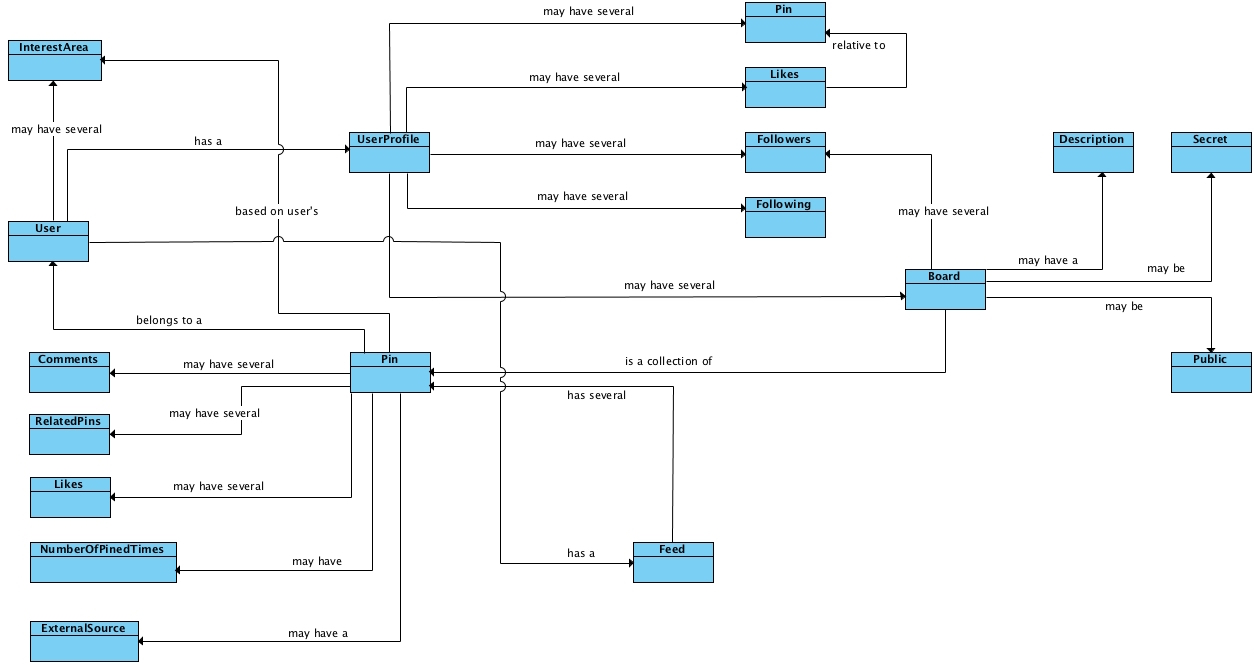
\includegraphics[width=1.20\textwidth]{img/pinterest-domain-model.jpg}
\caption{\label{img:pintdomain} Pinterest domain model schema.}
\end{figure}

\subsubsection*{Data Dictionary}
As one may notice from Figure \ref{img:pintdomain}, Pinterest introduces very particular concepts that may lack explanation, that is why we present first a small data dictionay before going trough the analysis, as we did with ResearchGate on a previous section:

\begin{itemize}
\item \textbf{Pin} - A Pin is the basic unit of Pinterest, it represents an idea of some user, presented in some context (the board context), and it is presented to us with a picture;
\item \textbf{Board} - As the name suggests, a board is a collection of pins. Boards are created from users to other users, and normally present pins within some context (e.g. travels, technology, food etc.). In Pinterest boards may be followed by other users;
\item \textbf{NumberOfPinedTimes} - This entity is not entirely a Pinterest entity, instead it represents a relevant metric introduced to measure pins popularity, and it refers to the act of saving pins. Pins that are presented to the users may be saved (or \textit{"pinned"}), and the number of times that users have saved a particular pin is expressed in Figure \ref{img:pintdomain} by the box \textit{NumberOfPinnedTimes};
\end{itemize}

\subsubsection*{Domain Model Analysis}
Pinterest introduces new concepts forming a very original \gls{osn}, because it's very different from others that we analyzed previously. Just as we seen in ResearchGate, where the domain model is build around a social object (the scientific publication), with Pinterest we have a similar scenario, where the concept of the platform is built around a different social object the Pin (\textit{Pin} box), which also as a grouped perspective introduced by a group or collection of pins that are the boards (\textit{Board} pin). Pinterest is basically a set of pins aggregated in boards that are explored in the platform accordingly to the user's interests.\\
\indent Simmilarly to other networks (e.g. Instagram) Pinterest also has direct unidirectional connections between users that adopt the concept of \textit{"follow/following"} (\textit{Followers} and \textit{Following} boxes). As user's can follow publications in ResearchGate, Pinterest users may follow boards, being then notified if some pin is added to that specific board.\\
\indent In what concerns to Pins, they may be commented by users (\textit{Comments} box), they also may be targeted by likes as posts in Facebook (\textit{Likes} box). A particular point concerning to Pins is that they can have a explicit external reference, for instance, if some image is extracted by some other web site or from other \gls{osn} they can be explicitly referenced, and that same reference appears at the top of the pin along with its title (\textit{ExternalSource} box).\\
\indent Pinterest was the traditional concept of feed, but in this case, the feed represents a completely different concept compared to other \gls{osn}. First the content of the feed (pins) is not related with users we follow on the network, is instead related is our personal interests (\textit{InterestArea} box) and second, they are not presented according to a chronological order, and visually they do not follow the standards of typical timeline/feed design, instead the different pins displayed on some user's feed, form some kind of board or catalog, like the ones people use to hang in walls and pin post-its on it.

\subsubsection*{Pinterest API}
According to \cite{pintdev}, Pinterest provides a REST API for developers interact with the platform. The data restrictions follow Facebook politics, where the application that integrates Pinterest API can only fetch data for authenticated users. Pinterest provides endpoints to interact with users, boards and pins. Concerning to the requests limitation, Pinterest offers a 60 minute sliding window where 1000 requests can be made by unique user token.

%% ---------------------------------------------- Exploring Some OSNs
%% -------------------------------------------------- SUMMARY?
